Так как, в нашем случае, лабораторный источник рентгеновского излучение имеет
некое угловое  (пучок не параллельный) и спектральное (характеристический спектр) распределение
для исследования материалов требуется наличие монохроматора, принцип действия которого
был описан в разделе \ref{sec:single_crystal_section}. Такой луч, отражаясь от
кристалла (схема на рис. \ref{ris:single_crystal_schem_lamtet}), разделятся в пространстве
в соответствие с условием Брегга (разные длины волн отражаются под разными углами).
В рамках последовательно движения от более простого к более сложному мы не оставили без внимание
получения угловой зависимости интенсивности (рисунок \ref{ris:single_crystal_schem_exp}), чтобы соотнести
выражение для описания спектра трубки (\ref{eq:source_spectral}) с экспериментальным.

\begin{figure}[H]
  \centering
  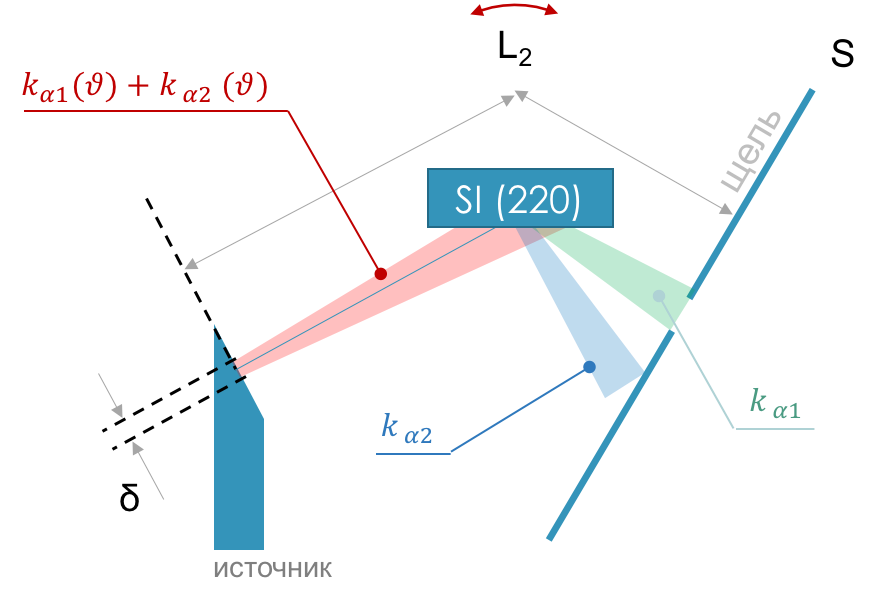
\includegraphics[width=0.5\textwidth]{images/single_crystal_schem_exp.png}
  \caption{Схема однокристального эксперимента, лучи с разной энергией отражаются под разными углами
  в соответсвии с условием Брегга}
  \label{ris:single_crystal_schem_exp}
\end{figure}

\begin{figure}[H]
  \centering
  \subfloat[$S = 50$ мкм; полуширина $k_{\alpha 1}$ линии ($\vartheta=0$)
  составляет около 30 угл.сек.]{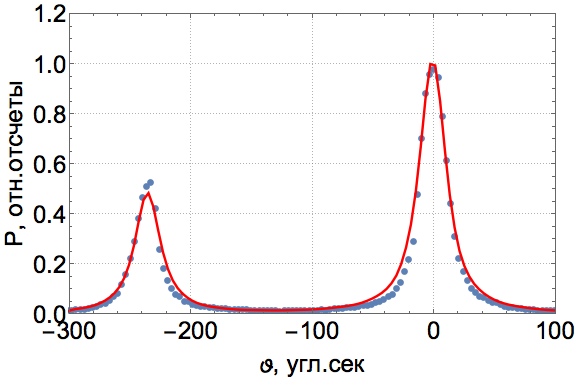
\includegraphics[width=0.45\textwidth]{images/single_cr_exp_s_005mm.png}}
  \hfill
  \subfloat[$S = 200$ мкм; полуширина $k_{\alpha 1}$ линии ($\vartheta=0$)
  составляет около 50 угл.сек.]{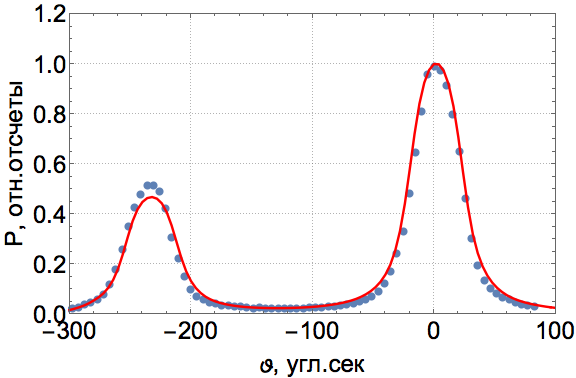
\includegraphics[width=0.45\textwidth]{images/single_cr_exp_s_02mm.png}}
  \caption{Однокристальный эксперимент проведенный для двух размеров щелевого устройства перед детектором,
   (красная линия) - расчет, (синие точки) - эксперимент. \textcolor{mygreen}{ по оси абсцисса - $\theta$ !} }
  \label{ris:zero_exp}
\end{figure}

Зависимость можно получить либо поворотом кристалла, либо движением щелевого устройства,
задающего апертуру детектора. В качестве кристалла был взят монокристалл кремния с отражающей
поверхностью (220).
